When thinking about finite tree automata, it is often desirable to have a
few simple examples in mind to compare classes.  We have collected a few
such examples here.

\subsection{Equalities Vs. Recursion}

\subsubsection{All-equal lists}

Not all classes of automata permit free interaction of recursion and
equality constraints; as such, these classes may not be able to describe the
language of all-equal lists: $\set{ [], [A], [A,A], [A,A,A], \ldots }$ for
any $A$.  Note, however, that for a fixed, regular tree $A$, the set of
all-equal lists of $A$ is a regular tree language.  The difficulty emerges
when we wish to describe all-equal lists over an unbounded number of
possible elements.

\subsubsection{Markovian-equal lists}

A generalization of the above, consider the language of lists composed of
regions of size at least two whose elements are equal, for example:
$[A,A,B,B,B]$ or $[A,A,A,B,B,C,C,D,D,D,D]$.  Rigid tree automata will not be
able to describe such a class due to the need for unboundedly many
equivalence classes.

\subsection{Opacity}

Consider the sets of trees described by
%
\begin{center}\begin{tabular}{cc}
    $\set{ f(g(X,Y),g(Z,X)) \middle\vert X,Y,Z \in \mathcal{T}(\Sigma)}$
  & $\set{ f(W,g(A,B)) \middle\vert A,B,W \in \mathcal{T}(\Sigma) \wedge A\vert_1 = B\vert_2 }$
  \\
    \begin{tikzpicture}
      \Tree [.f [.g X Y ] [.g Z X ] ]
    \end{tikzpicture}
  & \begin{tikzpicture}
      \Tree [.f W [.g$_{11=21}$ A B ] ]
    \end{tikzpicture}
\end{tabular}\end{center}
%
These descriptions are clearly (given their comprehension form) amenable to
classification by Opaque constraints.  Their intersection is $\set{
f(g(A,B),g(C,A)) \middle\vert A,B,C \in \mathcal{T}(\Sigma) \wedge C\vert_1
= A\vert_2 }$, which can be made amenable to Opaque classification only if
we are able to unfold $\mathcal{T}(\Sigma)$ for $A$ and $C$.  While we can
do this for regular trees over finite $\Sigma$, in general what we are
calling here $A$ will actually be trees accepted by a particular state, so
we can only describe this intersection with Opaque constraints if we are
able to unfold the description of that state.  In general, that unfolding
process might not terminate.
%
\Note{I would feel a lot better if somebody checked this.}

\subsection{Necessarily Overlapping}
\label{sec:tree-sepex:necessaryoverlap}

\begin{wrapfigure}{r}{1in}\centering\begin{tikzpicture}
  \Tree [.f$_{1=22}$ X [.g$_{1=2}$ X X ] ]
\end{tikzpicture}\end{wrapfigure}
The tree in the figure to the right is a small example of a structure which
necessarily involves overlapping constraints, assuming that the nodes
$X$ are drawn from an infinite set of trees; if there are merely finitely
many possibilities, then the constraints may be pushed into the state
label.  Specifically, because we must constrain positions $1$, $21$ and $22$
to be equal, we are obligated to have at least one of $21$ and $22$ as
constraint paths in the automata, and then either the other, which overlaps,
or the constraint $1=2$ at position $2$, which again overlaps.  However,
this structure is amenable to Opaque description, as shown.

\subsection{Two-counter decomposition}

Many classes admit machines which, when intersected, yield the two-counter
example of \cite{tata}.%
%
\footnote{\Note{Somewhere, possibly here, more should be said about this
excellent example.  A concise summary of how it does what it does is that
the right spine is the whole computation history and each entry thereon
carries two complete copies, offset by one move, of its computational path
prefix, or provenance.}}
%
For concreteness, we give a set of five such machines.  In all cases, $q_f$
is the accepting state.  These machines encode overlapping supersets of the
set of trees encoding valid two-counter machine execution traces; their
intersection is exactly this language.  \begin{itemize}
%
  \item The ``end-state'' machine specifies only the left subtree of the
  root $h$ node: it requires that the encoding's state label be that of the
  accepting state of the underlying 2CM.
%
  \item The ``structural equality and initial-state'' machine specifies more
  structure: it demands that the tree be a right-branching non-empty list,
  using $h/2$ as cons and $\#$ as nil, whose ultimate member must encode the
  initial state of the underlying 2CM with zeroed counters.  Each other
  element of this list must be a structure unifying $g(P,h(g(P',X),X))$
  where $P$ and $P'$ are possible 2CM encodings.
%
  \item The ``top-level constraint'' machine encodes all trees which unify
  with $h(g(X,Y),Y)$.
%
\end{itemize} Not shown here are two more machines along the same lines as
the ``structural equality and initial-state'' machine, but which impose
different equality constraints and mandate relations between the
configurations of the underlying 2CM, corresponding to the rules of said
2CM.

Note that each of these machines, taken in isolation, satisfies a slew of
local metaconstraints: Reducing (each machine has at most two ranks), Stated
(because they are all single-ply), $rank$-same-stated, $id$-same-stated
\Note{Please check two not pictured}, Opaque, and Non-overlapping.  Further,
all these machines are equivalent to multi-ply machines additionally
satisfying Contained. \Note{I believe this is right for the two not
pictured, as well.}  Due to the presence of $q_\forall$, none of them are
deterministic machines.  We may therefore conclude that (at least) any class
of nondeterministic machines which is subject to any subset of these
metaconstraints and does not impose additional restrictions {\em has at most
one of decidable emptiness testing and closure under intersection}.

\begin{lrbox}{\tempboxa}
\begin{minipage}{4cm}
\begin{align*}
  h(g_q, q_\forall) &\rightarrow q_f \\
  g(q_a, q_\forall) &\rightarrow q_g \\
  p_{accept}(q_{\mathbb{N}}, q_{\mathbb{N}}) &\rightarrow q_a \\
  z &\rightarrow q_{\mathbb{N}} \\
  s(q_{\mathbb{N}}) &\rightarrow q_{\mathbb{N}}
\end{align*}
\end{minipage}
\end{lrbox}
\begin{lrbox}{\tempboxb}
\begin{minipage}{3cm}
\begin{align*}
  h(q_g, q_\forall) &\xrightarrow{12=2} q_f \\
  g(q_\forall, q_\forall) &\rightarrow q_g
\end{align*}
\end{minipage}
\end{lrbox}
\begin{lrbox}{\tempboxc}
\begin{minipage}{3cm}
\begin{align*}
  g(q_p, q_h) &\xrightarrow{22=212} q_g \\
  h(q_g', q_\forall) &\rightarrow q_h \\ 
  g(q_p, q_\forall) &\rightarrow q_g' \\
  \forall i . p_i(q_{\mathbb{N}}, q_{\mathbb{N}}) &\rightarrow g_p \\
  z &\rightarrow q_{\mathbb{N}} \\
  s(q_{\mathbb{N}}) &\rightarrow q_{\mathbb{N}}
\end{align*}
\end{minipage}
\end{lrbox}
\begin{lrbox}{\tempboxd}
\begin{minipage}{3cm}
 \begin{align*}
  h(q_g, q_\#) &\rightarrow q_f \\
  g(q_i, q_\#) &\rightarrow q_g \\
  p_{init}(q_z, q_z) &\rightarrow q_i \\
  \# &\rightarrow q_\# \\
  z  &\rightarrow q_z
\end{align*}
\end{minipage}
\end{lrbox}

\begin{tabular}{|c|c|c|}
\hline
{End state $p_{accept}$} &
{Top-level constraint} &
{Structural equality and base}
\\
\hline
\Tree [.h [.g [. p$_{accept}$ N$_l$ N$_r$ ] Y ] Z ]
&
\Tree [.h$_{12=2}$ [.g X Y ] X ]
&
\Tree [.h [.g$_{22=212}$ [.p$_j$ $N'_l$ $N'_r$ ] [.h [.g [.p$_{1i}$ $N_{1l}$ $N_{1r}$ ] X$_1$ ] $Y_1$ ] ] [.$\cdots$ $\cdots$ [.h [.g [.p$_{init}$ z z ] [.\# ] ] [.\# ] ] ] ]
\\
\hline

\usebox{\tempboxa}
&\usebox{\tempboxb}
&
{
	\begin{tabular}{cc}
    	\multicolumn{2}{c}{$h(q_T,q_f) \rightarrow q_f$} \\
		\usebox{\tempboxc} & \usebox{\tempboxd}
	\end{tabular}
}
\\
\hline
\end{tabular}
